% GENERATED by scripts/workflow_centreline_panels.py -- do not edit by hand.
% 4x4 grid of frame-space panels: rows are the ground-truth vessel count 0..3,
% columns are the four models, and the key spans the grid on the right. Axes are
% drawn once per edge (left column, bottom row) and their margins hang outside the
% grid, so the plot boxes stay flush. The block's top-left corner is (0, 0) and it
% grows right and down; (fgtl) and (fgbr) mark its corners for a fit= group node.
\coordinate (fgtl) at (0, 0);
\coordinate (fgbr) at (25.706, -20.078);
\node[bimg] (fg00) at (0.800, -0.850) {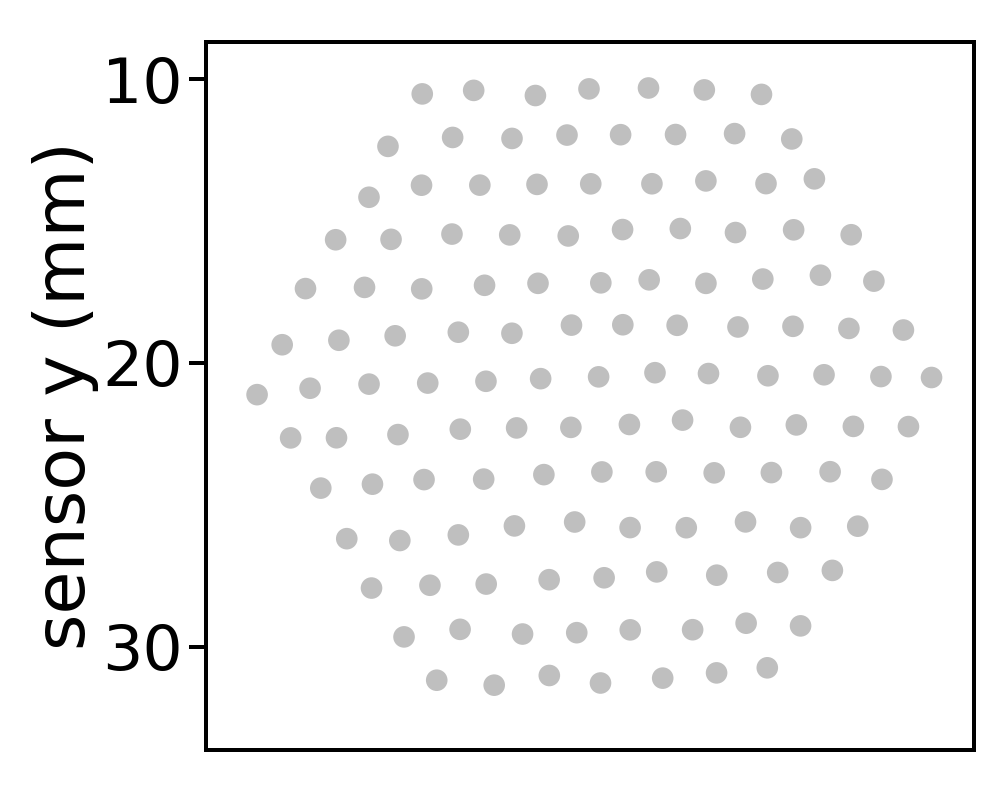
\includegraphics[width=5.394cm]{workflow/cl_grid_0_sim_to_sim.png}};
\node[bimg] (fg01) at (6.474, -0.850) {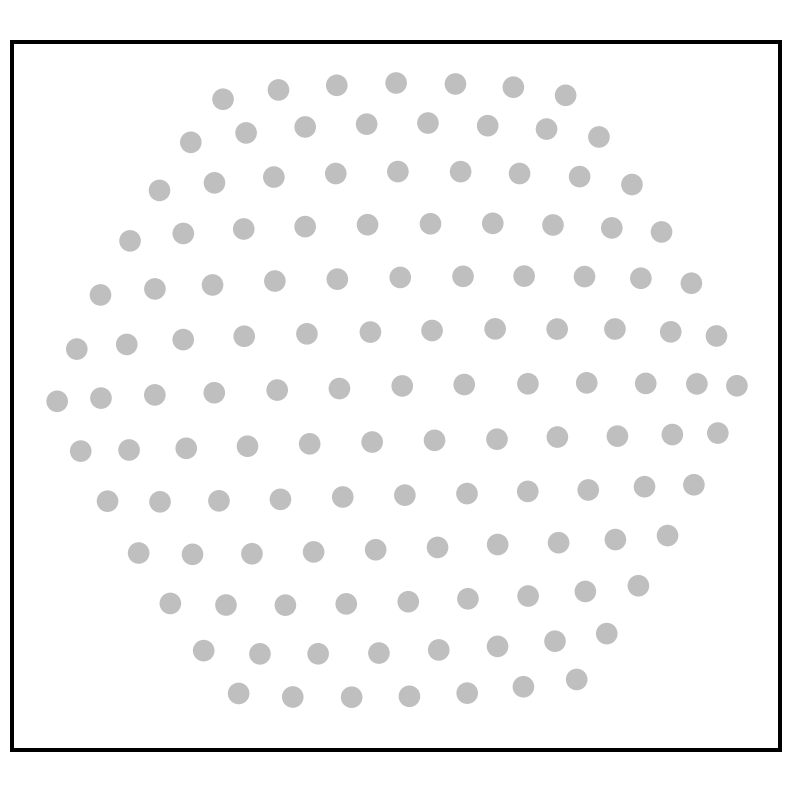
\includegraphics[width=4.331cm]{workflow/cl_grid_0_sim_to_silicone.png}};
\node[bimg] (fg02) at (11.086, -0.850) {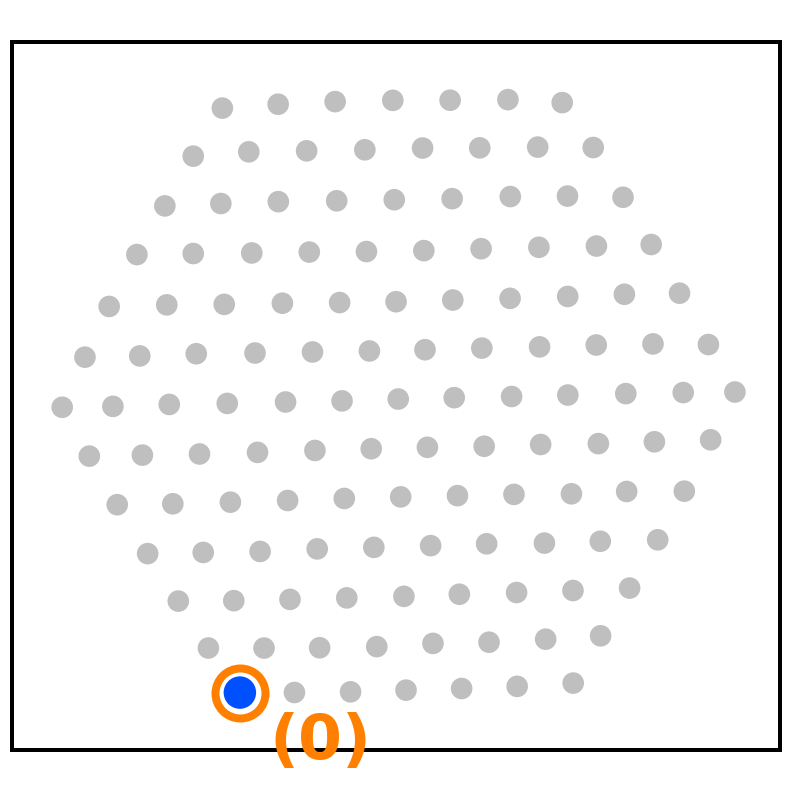
\includegraphics[width=4.331cm]{workflow/cl_grid_0_sim_to_meat.png}};
\node[bimg] (fg03) at (15.697, -0.850) {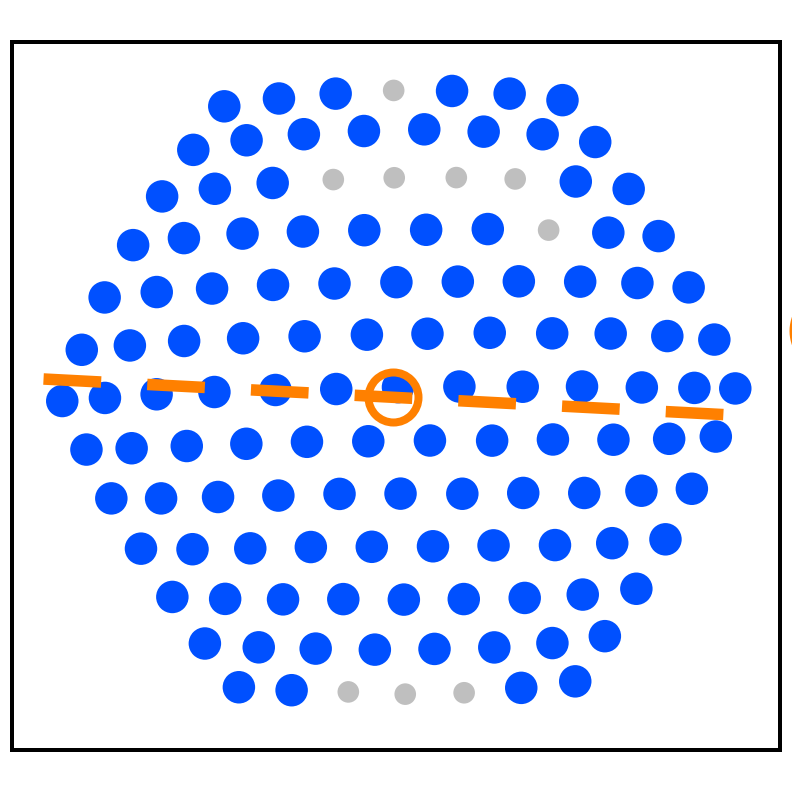
\includegraphics[width=4.331cm]{workflow/cl_grid_0_meat_to_silicone.png}};
\node[bsub, rotate=90, anchor=south] at (0.700, -3.016) {0 vessels};
\node[bimg] (fg10) at (0.800, -5.461) {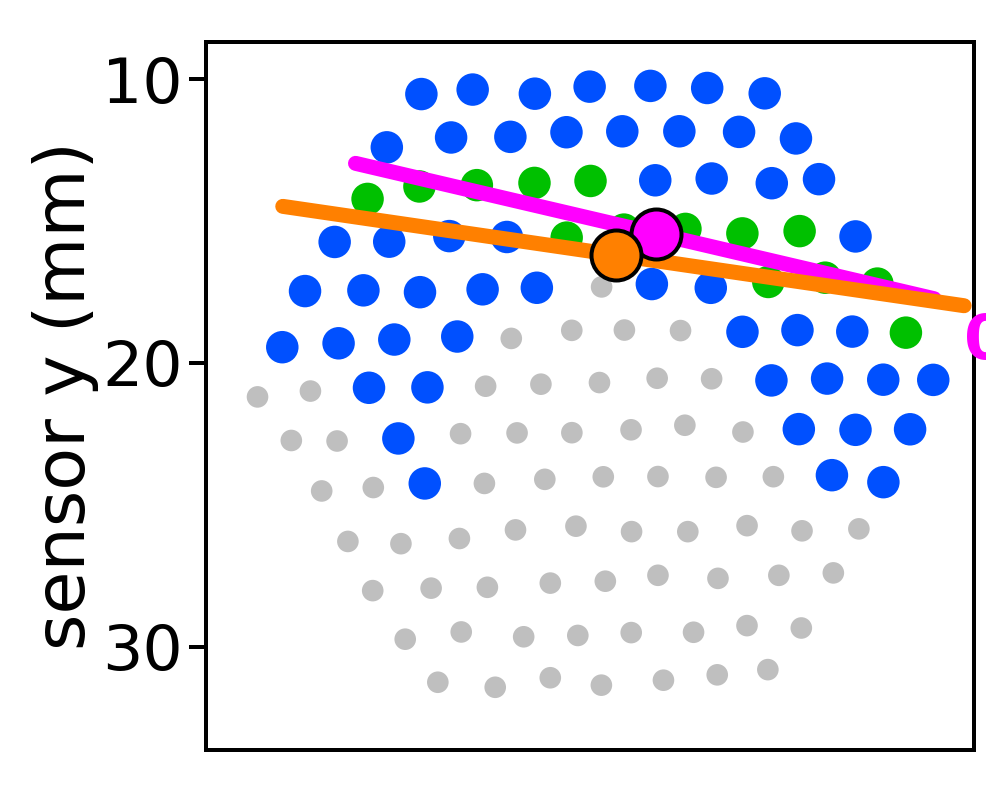
\includegraphics[width=5.394cm]{workflow/cl_grid_1_sim_to_sim.png}};
\node[bimg] (fg11) at (6.474, -5.461) {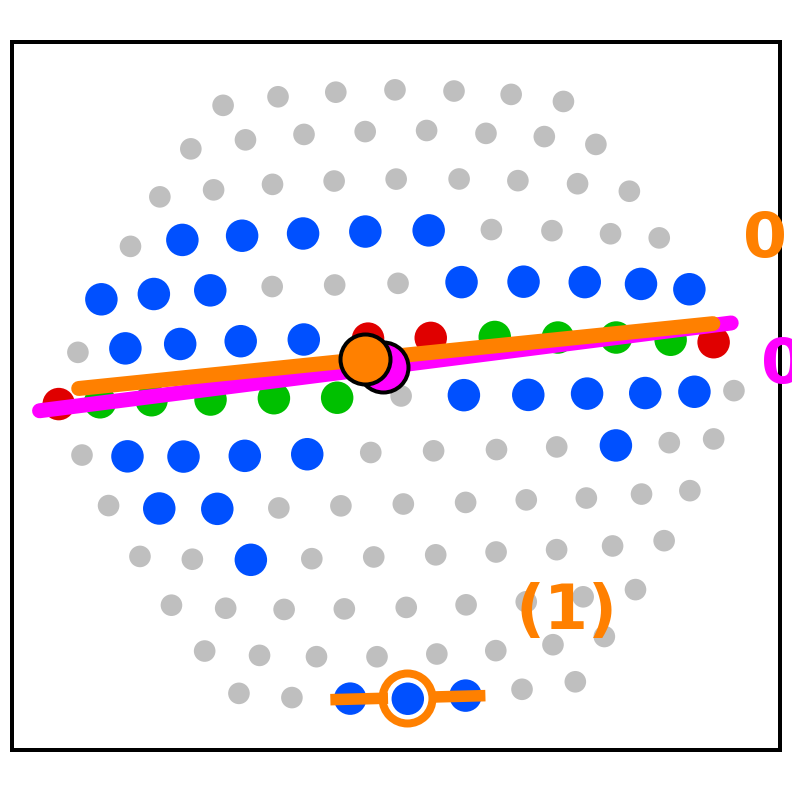
\includegraphics[width=4.331cm]{workflow/cl_grid_1_sim_to_silicone.png}};
\node[bimg] (fg12) at (11.086, -5.461) {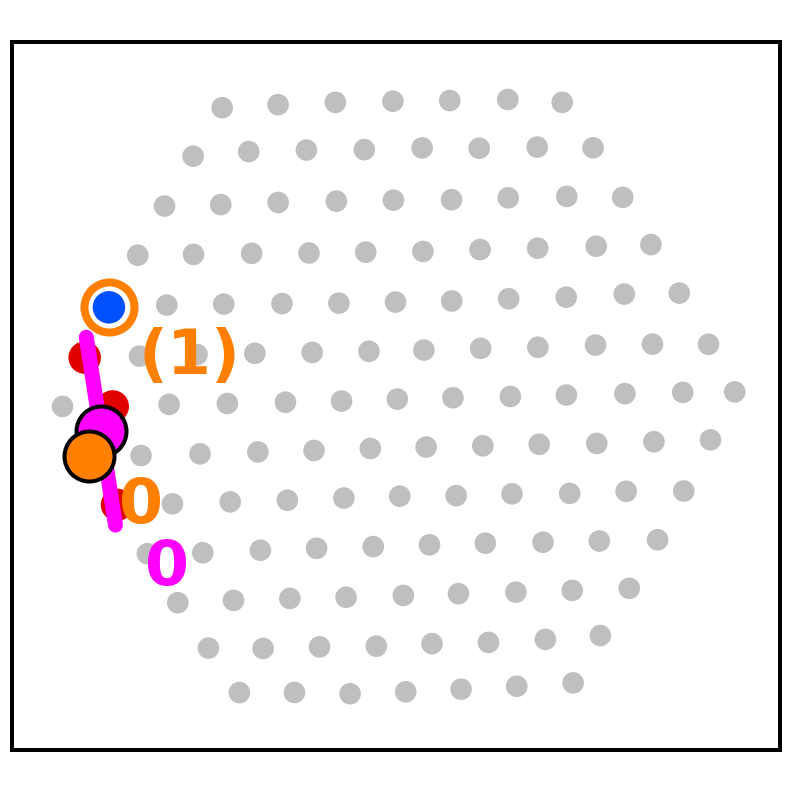
\includegraphics[width=4.331cm]{workflow/cl_grid_1_sim_to_meat.png}};
\node[bimg] (fg13) at (15.697, -5.461) {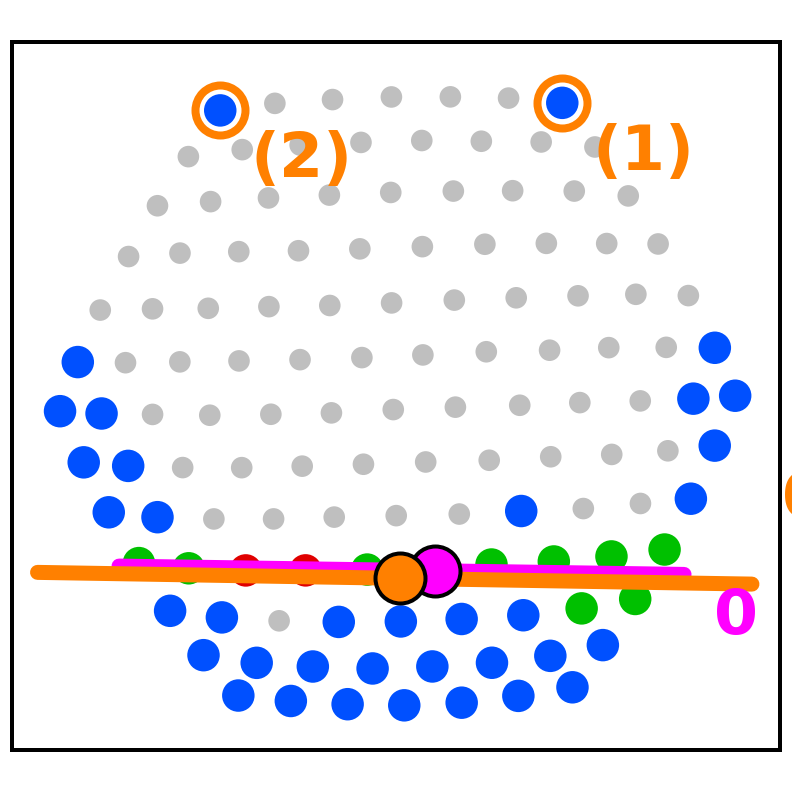
\includegraphics[width=4.331cm]{workflow/cl_grid_1_meat_to_silicone.png}};
\node[bsub, rotate=90, anchor=south] at (0.700, -7.627) {1 vessel};
\node[bimg] (fg20) at (0.800, -10.072) {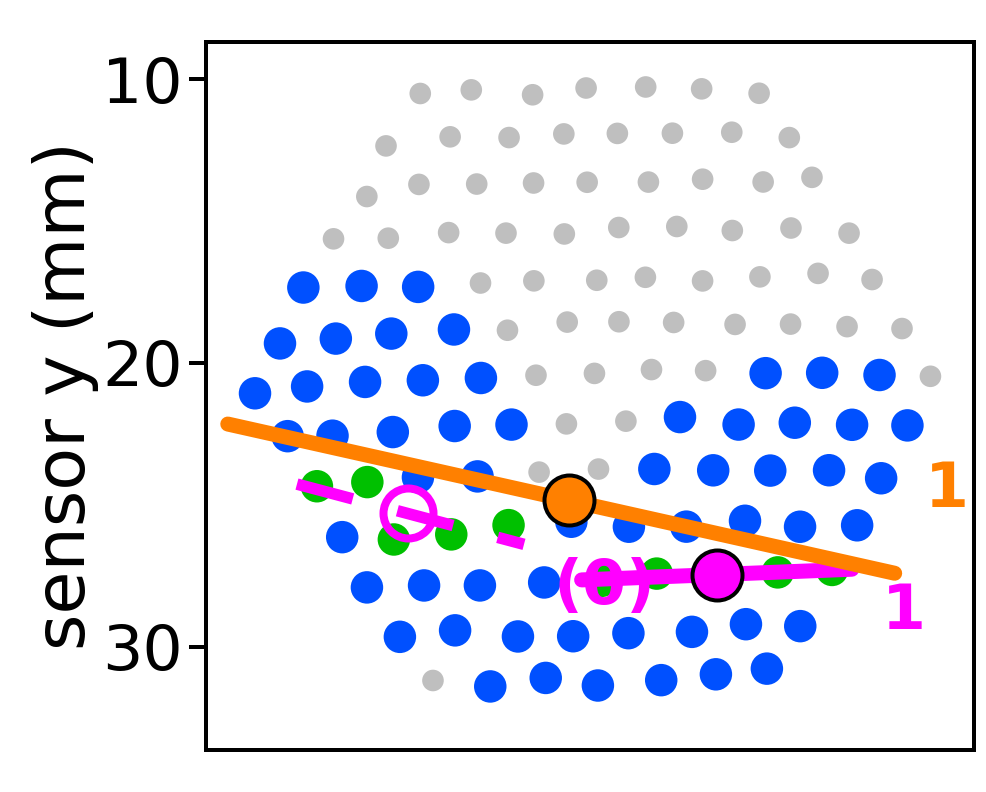
\includegraphics[width=5.394cm]{workflow/cl_grid_2_sim_to_sim.png}};
\node[bimg] (fg21) at (6.474, -10.072) {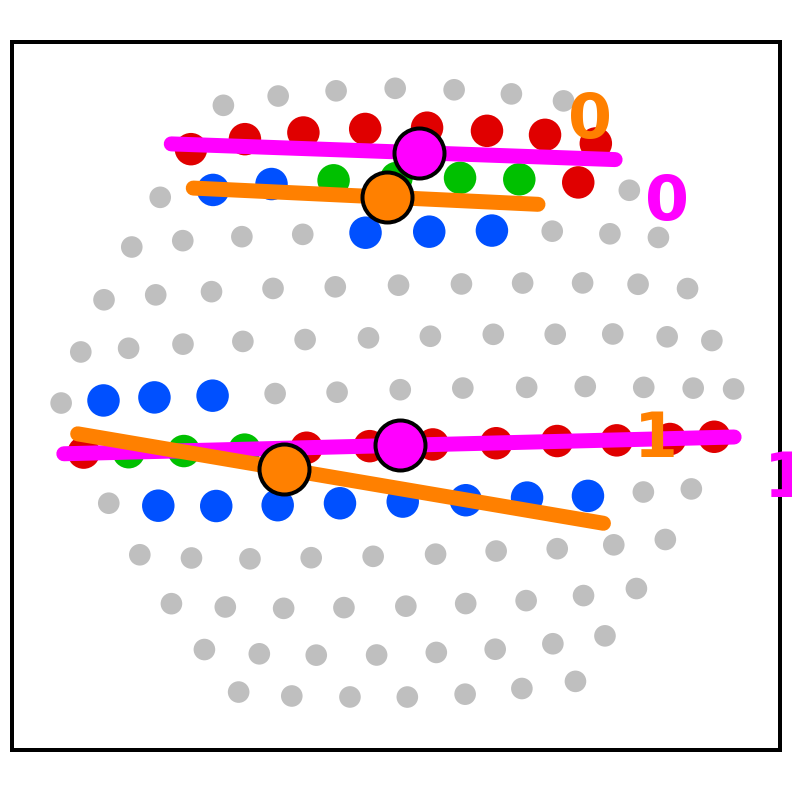
\includegraphics[width=4.331cm]{workflow/cl_grid_2_sim_to_silicone.png}};
\node[bimg] (fg22) at (11.086, -10.072) {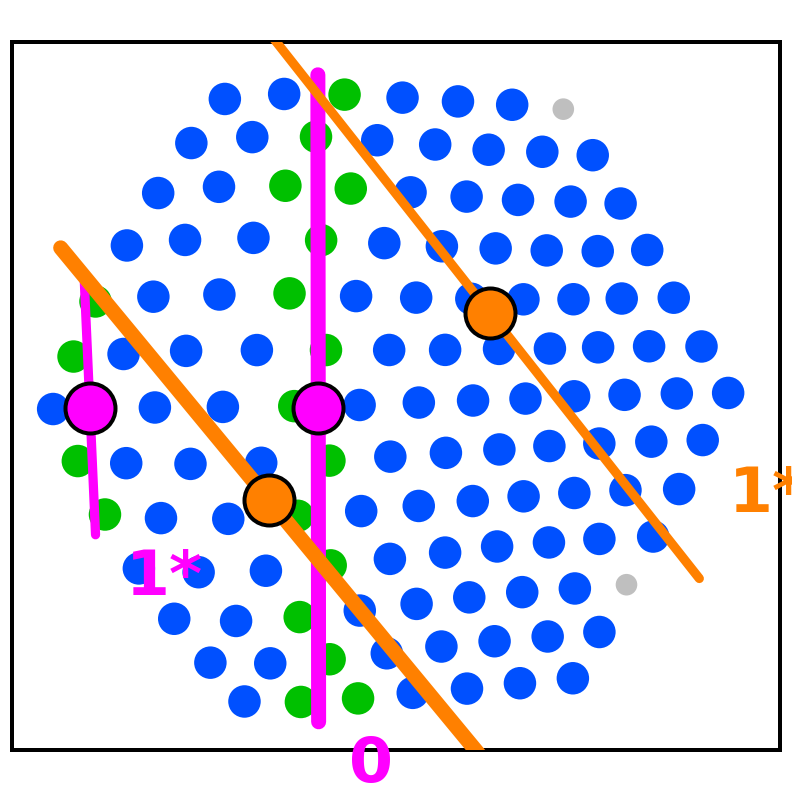
\includegraphics[width=4.331cm]{workflow/cl_grid_2_sim_to_meat.png}};
\node[bimg] (fg23) at (15.697, -10.072) {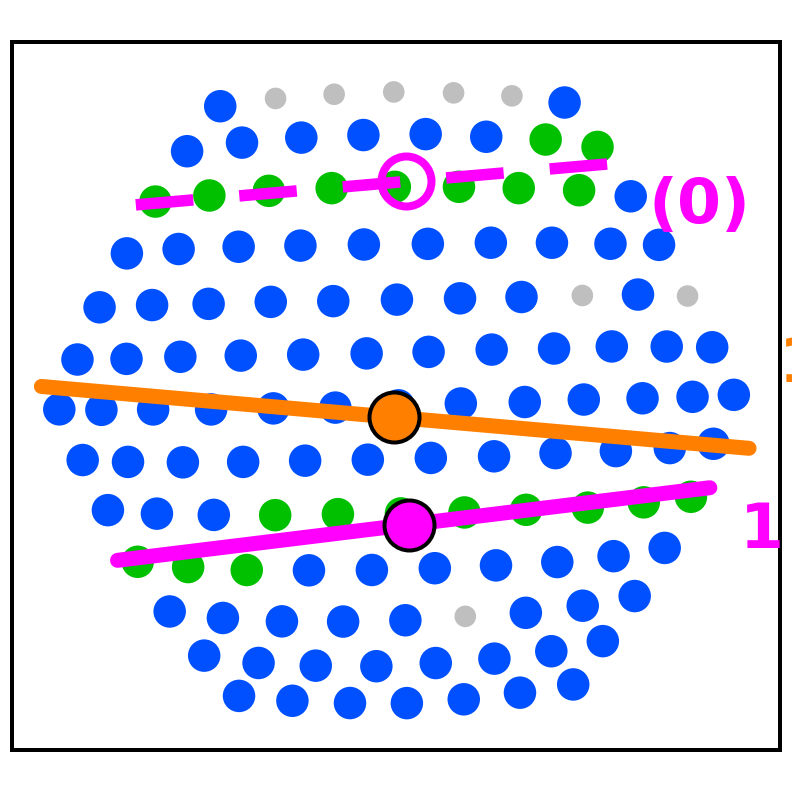
\includegraphics[width=4.331cm]{workflow/cl_grid_2_meat_to_silicone.png}};
\node[bsub, rotate=90, anchor=south] at (0.700, -12.238) {2 vessels};
\node[bimg] (fg30) at (0.800, -14.684) {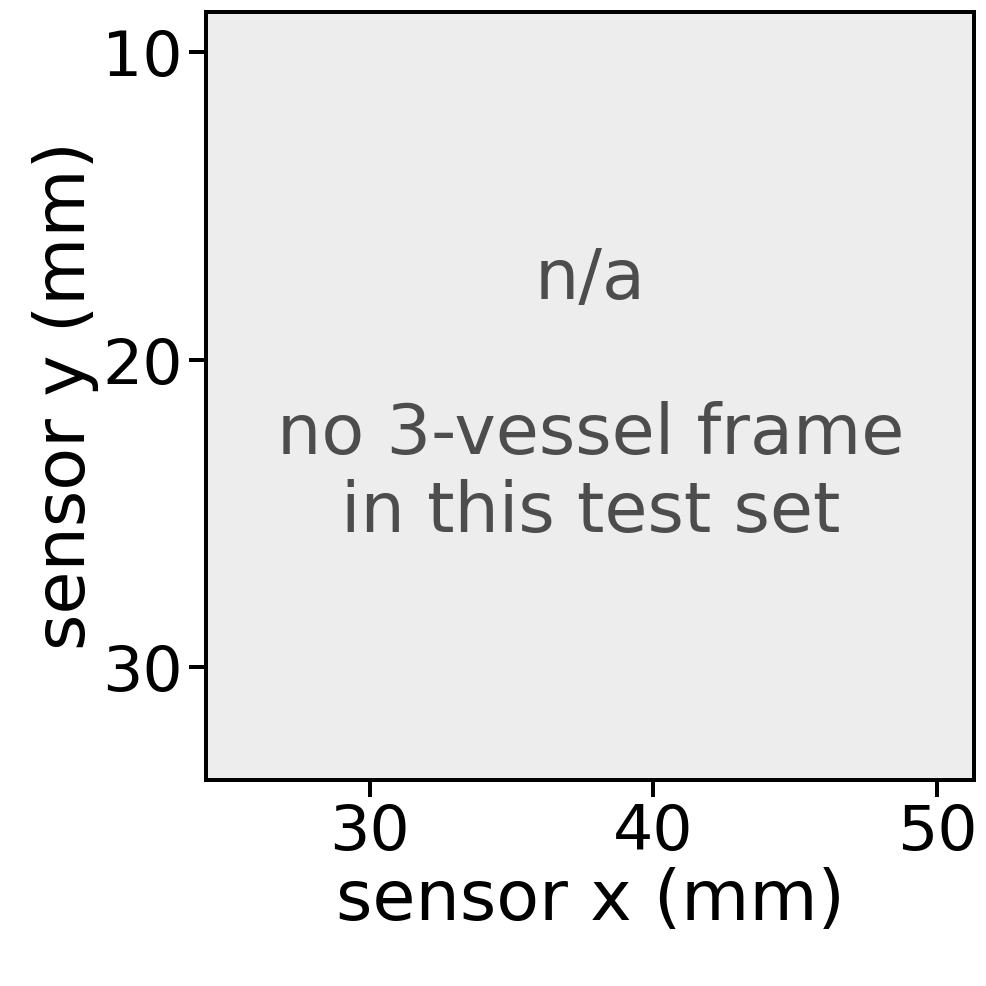
\includegraphics[width=5.394cm]{workflow/cl_grid_3_sim_to_sim.png}};
\node[bimg] (fg31) at (6.474, -14.684) {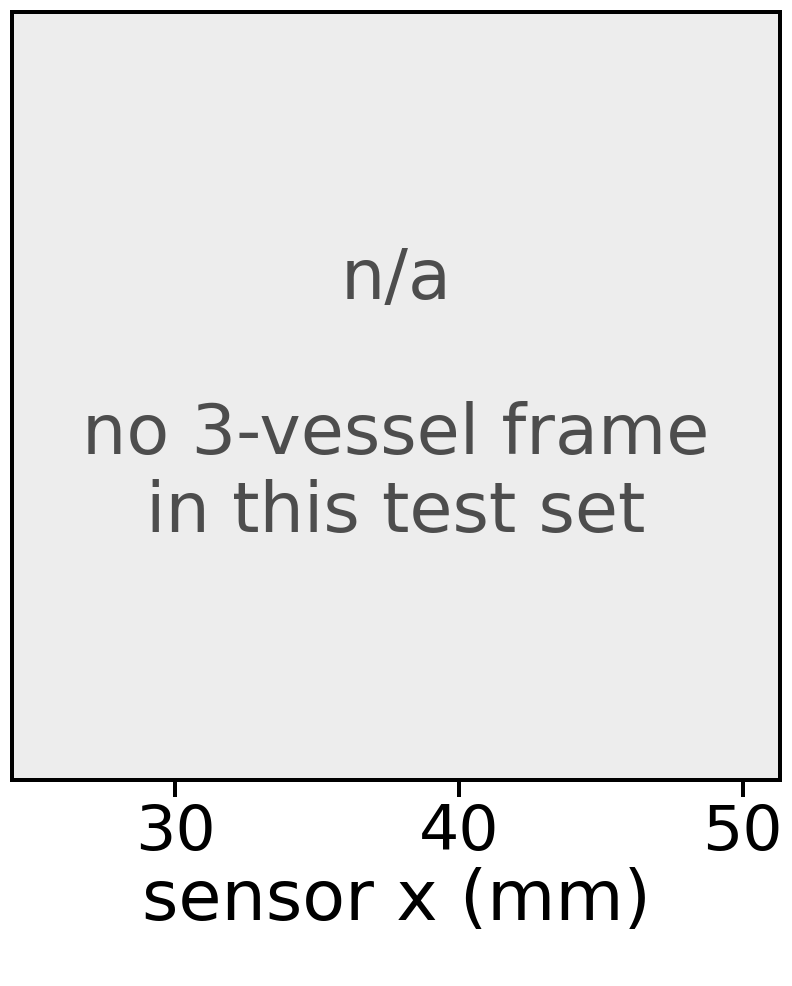
\includegraphics[width=4.331cm]{workflow/cl_grid_3_sim_to_silicone.png}};
\node[bimg] (fg32) at (11.086, -14.684) {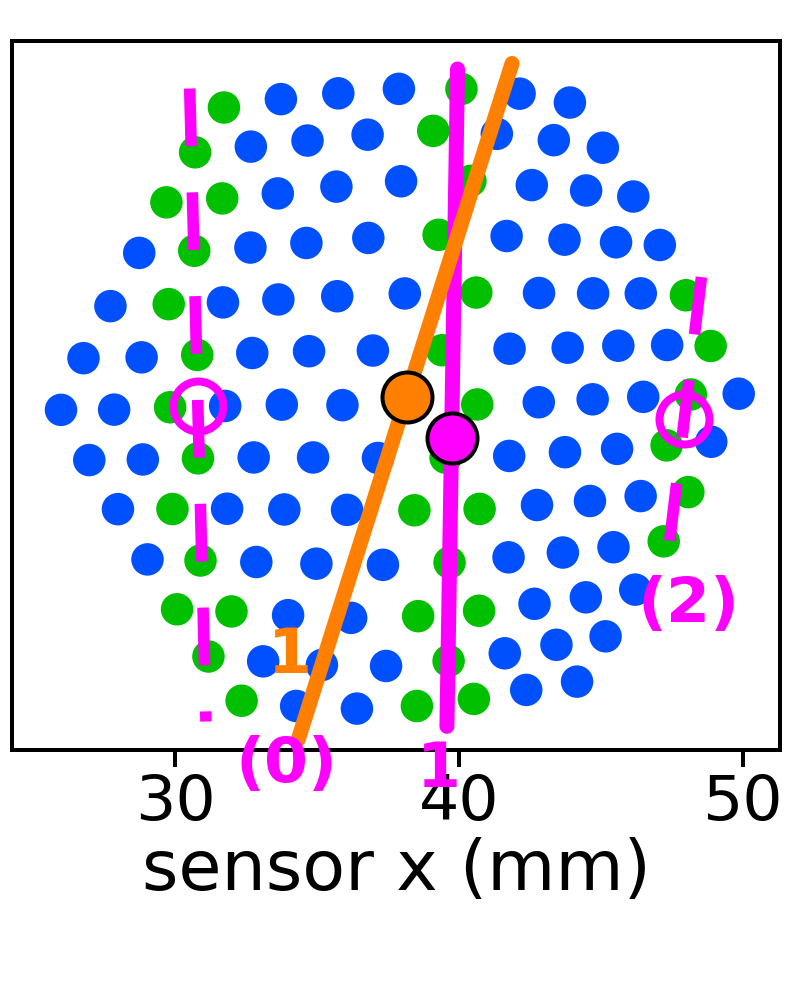
\includegraphics[width=4.331cm]{workflow/cl_grid_3_sim_to_meat.png}};
\node[bimg] (fg33) at (15.697, -14.684) {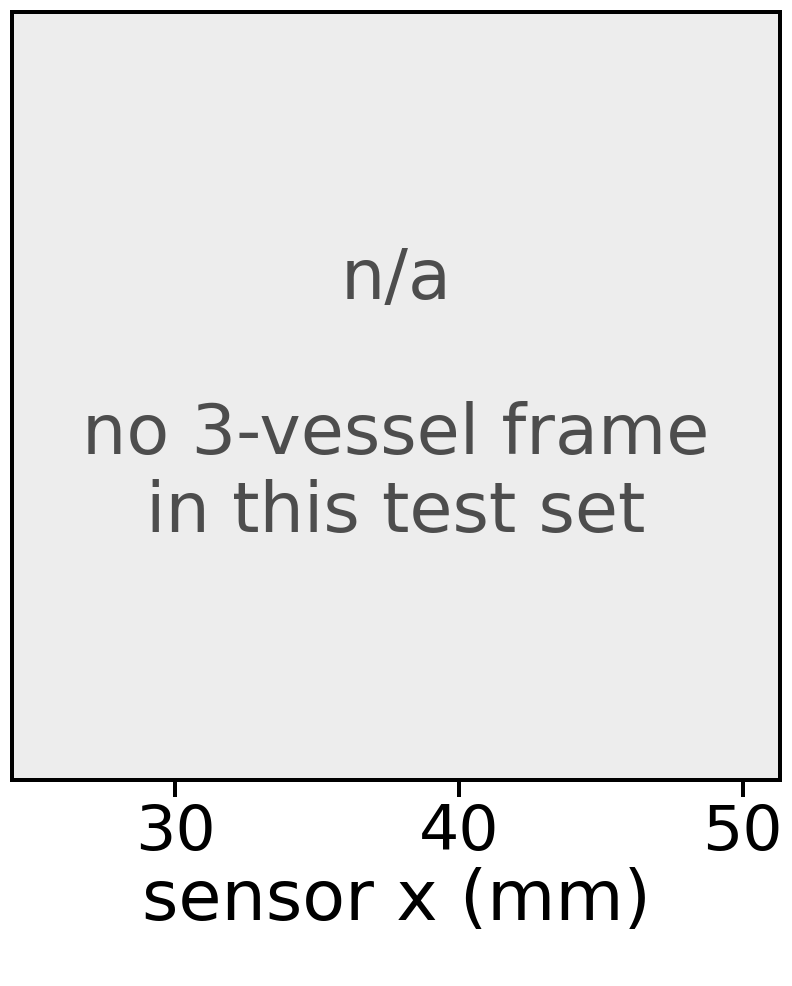
\includegraphics[width=4.331cm]{workflow/cl_grid_3_meat_to_silicone.png}};
\node[bsub, rotate=90, anchor=south] at (0.700, -16.849) {3 vessels};
\node[bsub, anchor=south] at (4.029, -0.730) {\msq{MdlA}~Sim$\rightarrow$Sim};
\node[bsub, anchor=south] at (8.640, -0.730) {\msq{MdlB}~Sim$\rightarrow$Silicone};
\node[bsub, anchor=south] at (13.251, -0.730) {\msq{MdlC}~Sim$\rightarrow$Meat};
\node[bsub, anchor=south] at (17.862, -0.730) {\msq{MdlD}~Meat$\rightarrow$Silicone};
\node[bimg] (fgkey) at (20.658, -0.850) {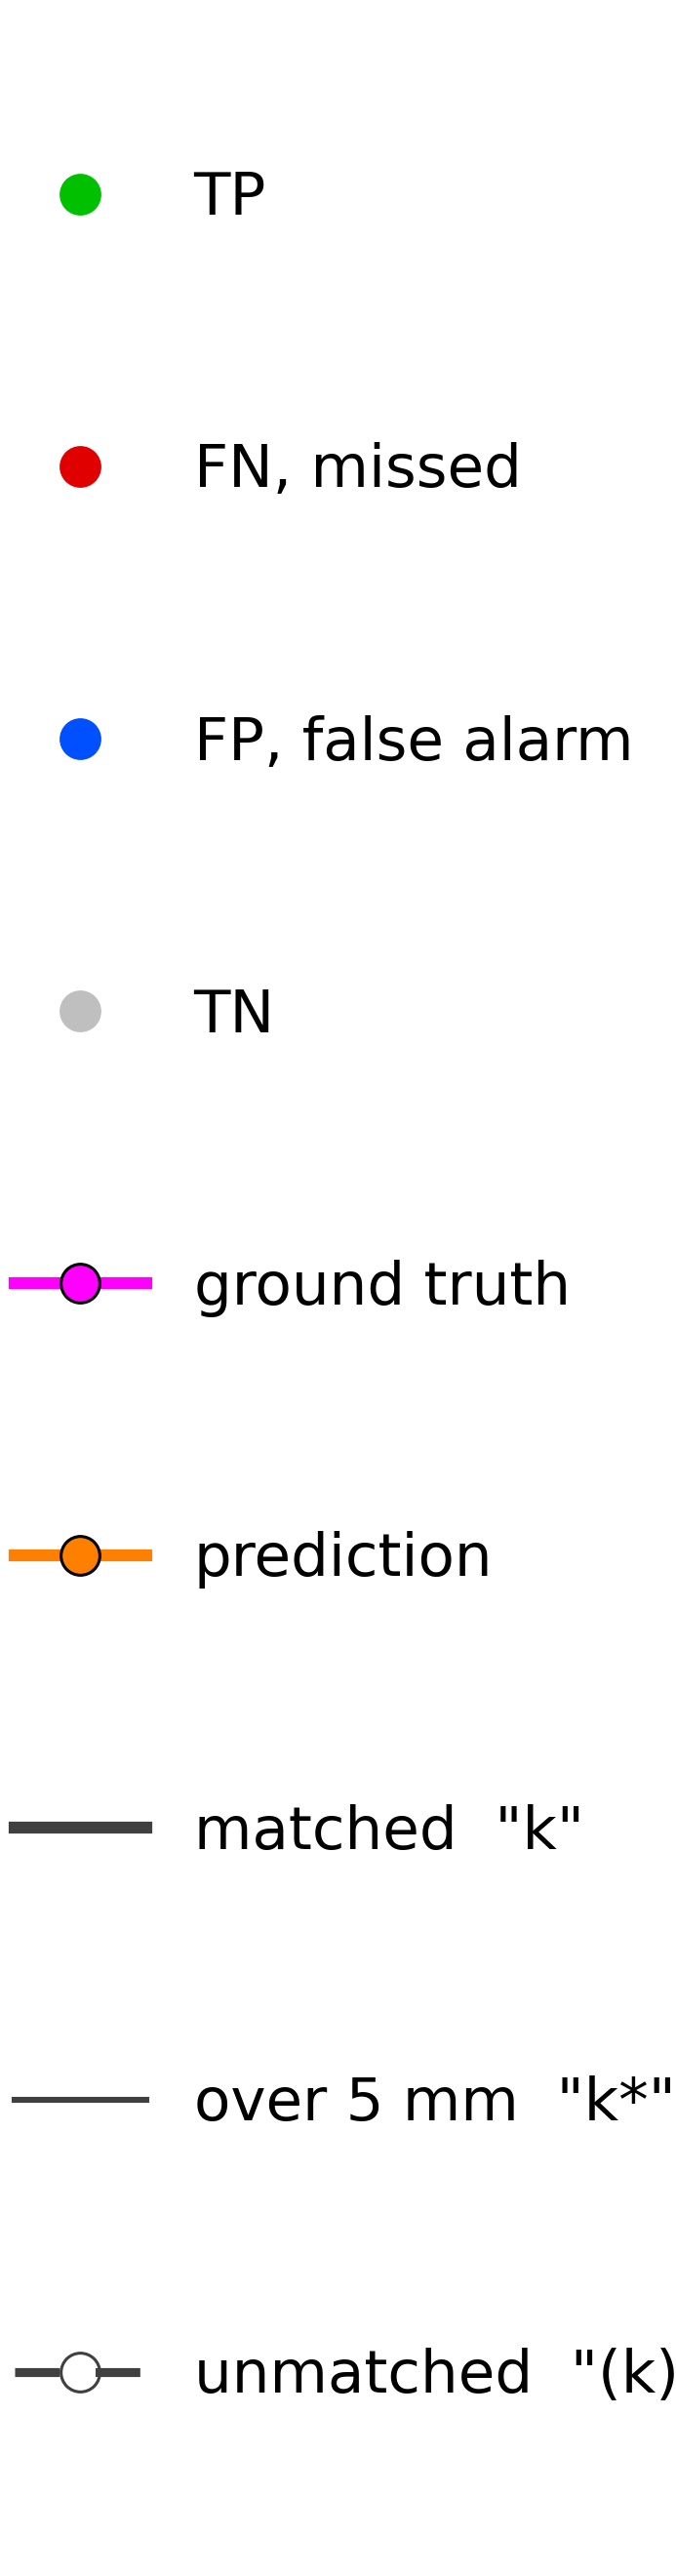
\includegraphics[height=19.228cm]{workflow/cl_legend.png}};
